\section{The Equations of Least Squares}
This chapter presents the essential mathematics for global positioning. In the big picture,
we have measurements of the pseudoranges from satellites to receivers. With so many
satellites we expect to have more measurements than the minimum to determine X, Y, Z, t
(position and time). But those measurements contain errors(so we use the expression
“pseudo” for observed distances). This is exactly the context of least-squares algorithms:
to find the best solution to inconsistent equations.

The model problem is an overdetermined linear system with noise e(error): 
\begin{equation}\label{eq:4.1}
Ax=b-e
\end{equation}
Typically we have m equations (m observations) to fit by n parameters. ( The unknowns
$x_1,x_2,...,x_n$ can represent position or velocity or time at the receivers.) The equations
$Ax=b$ are expected to have no solution, because m$>$n. Our task is to find a best
solution $\hat{x}$( called “x hat ”).

This chapter establishes the equations that determine $\hat{x}$ when the noise vector e is
taken to be a random variable. Start with the simplest assumption: The m components of e
come independently from standard normal distributions(mean 0 and variance 1). There is
no reason to trust any equation in $Ax=b$ less or more than any other. The unweighted
least-squares solution minimizes$\| b-Ax \|^2$, the sum of squared errors. The best estimate $\hat{x}$ solves the normal equations
\begin{equation}\label{eq:4.2}
A^TA\hat{x}=A^Tb
\end{equation}
We will derive these equations by calculus and by geometry and algebra. Calculus minimizes $E=\|b-Ax\|^2$ by the usual conditions $\partial E/\partial x_i=0$. Geometry minimizes E by
choosing the combination $A\hat{x}$ of the columns of A that is closest to b . Algebra recognizes
this Ax $A\hat{x}$ as the projection of b onto the subspace of all possible combinations Ax.

All ways of understanding the normal equations $A^TA\hat{x}=A^Tb$ deserve your attention. Perhaps this is the most important application of linear algebra.

Solving these equations numerically is a separate question. In most cases we simply form the coefficient matrix $A^TA$ (symmetric and positive definite), and then solve by
elimination without pivoting. But it can well happen that this is not the optimal way:

1. Greater numerical stability may be needed when $A^TA$ is ill-conditioned (the columns
of A are nearly dependent). Then a “square root method” avoids forming $A^TA$.
Instead the columns of A can be orthogonalized in advance — this is described in
Chapter 5. The famous algorithm uses the Gram-Schmidt method, but Householder
matrices give a better way. And the SVD can play its important part.

2. The observations in b may not arrive all at once. In this case we prefer recursive least
squares, which updates the estimated $\hat{x}$ to reflect the latest observations — without
repeating earlier steps and recomputing from the start.

In dynamic applications (such as a moving receiver) the state itself is changing. We
are estimating a different position vector $x_i$ from the new observations at step i. But
this $x_i$ is related to the previous $x_(i-1)$ by a state equation. So there is a two-stage
process at each step: a prediction from the state equation (which has its own error
sources) followed by a correction to account for the new observations at that step.

The Kalman filter executes those two steps. We explain the ideas and derive the
update formulas in Chapter 8, after an example in Section 4.3.

3. The m observations in b may not be equally reliable (and they may not be independent, the errors $e_1,...,e_m$ could be correlated). The uncertainties in the $b_i$ are measured by variances of $\sigma^2_i$. The correlations of $e_i$ with $e_j$ are measured by covariances $\sigma_ij$. All these numbers enter the “covariance matrix” $\Sigma$ , described below. 

This symmetric matrix $\Sigma$ tells us the correct weights for the observation equations
$Ax=b$. Ordinary least squares has the implicit assumption that $\Sigma=\sigma^2I$, independence with equal variances leading to equal weights. An equation with a larger
variance is less reliable and should have smaller weight.  

We vvill show how the inverse matrix $C=\Sigma^-1$ is the correct choice for weighted
least squares. The normal equations change from $A^TA\hat{x}=A^Tb$ to $A^TCA\hat{x}=A^TCb$. These are the equations to solve, directly or recursively. And the crucial output is not only the best estimate $\hat{x}$ but also the covariance matrix $P=(A^TCA)^-1$
for the reliability of that best estimate.

This chapter explains probability distributions and covariances. The normal (or Gaussian ) with the factor $e^-|x|^2 /2$ is always dominant. That exponent becomes$-x^TCx/2$ when the covariance matrix $\Sigma=C^-1$ is included. These are fundamental ideas, and their applications to positioning are the centerpiece of this book.

Example 4.1 A crucial application of least squares is fitting a straight line to m points.
Start with three points: Find the closest line to the points (0,6), (1,0), and (2,0). 

\begin{figure}[h]
	\centering
	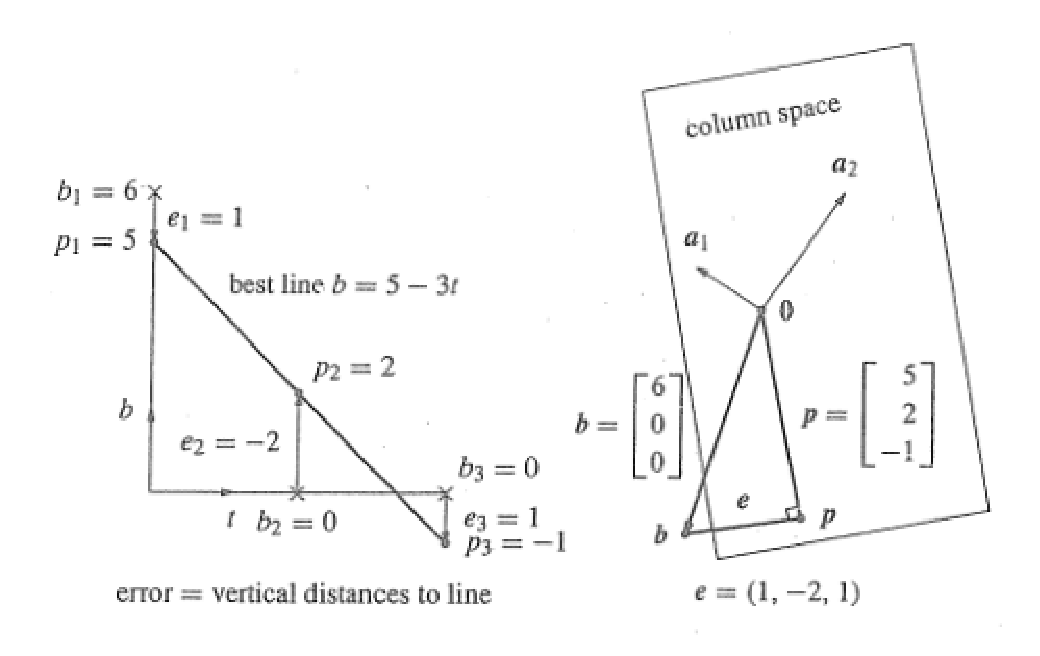
\includegraphics[width=0.7\linewidth]{TeX_files/Part02/chapter04/image/4-1}
	\caption{}
	\label{fig:4-1}
\end{figure}

Figure 4.1  Best line and projection: Two pictures, same problem. The line has heights p=(5,2,—1) with errors e=(1,—2,1) . The equations $A^TA\hat{x}=A^Tb$ give $\hat{x}=(5,-3)$.The best line is 5-3t. In the second picture, b is projected to $p=5a_1-3a_2$.

No straight line b= C + Dt goes through those three points. We are asking for two
numbers C and D that satisfy three equations. Here are the equations at t = 0,1,2 to
match the given values b = 6,0,0:

t = 0 The first point is on the line b = C + Dt  \quad\quad if\;  $C+D*0=6$ 

t = 1 Tne second point is on the line b = C + Dt \quad if\;  $C+D*1=0$

t = 2 The third point is on the line b = C + Dt  \quad\quad if\;  $C+D*2=0$.

This 3 by 2 system has no solution: b=(6,0,0) is not a combination of the columns
(1,1,1) and (0,1,2). Read off A, x, and b from those equations and solve $A^TA\hat{x}=A^Tb$:

\begin{equation*}
A=              
\begin{bmatrix}
1 & 0 \\ 1 & 1 \\ 1 & 2
\end{bmatrix}
\ x=
\begin{bmatrix}
C \\ D
\end{bmatrix}
\ b=
\begin{bmatrix}
6 \\ 0 \\0
\end{bmatrix}
\quad Ax=b \:is \,not \,solvable.	
\end{equation*}

	\subsection{Minimizing the Error}
	How do we make the error e = b - Ax as small as possible ? This is an important question
	with a beautiful answer. The best x (called$\hat{x}$) can be found by geometry or algebra or
	calculus: 90 ° angle, or project the vector by or set derivatives of the squared error to zero.
	
	By geometry Every Ax lies in the plane of the columns (1,1,1) and (0,1,2). In that plane
	(Figure 4.1), we look for the point closest to b. The nearest point is the projection p.
	
	The best choice for $A\hat{x}$ is p. The smallest possible error is e = b - p . The three
	points at heights $(p_1,p_2,p_3)$ do lie on a line, because p is a combination of the two
	columns with coefficients C and D. In fitting a straight line, $\hat{x}$ gives the best choice for (C, D ).
	
	By algebra Every vector b splits into two parts. The part in the column space is p. The
	perpendicular part in the nullspace of $A^T$ is the error e . There is an equation we cannot
	solve (Ax = b). There is an equation $A\hat{x}=p$ we do solve (by removing e).
	
	\begin{equation}
	Ax = b = p + e \;is\,impossible;  \quad  A\hat{x} = p \;is\,solvable;
	\end{equation}   
	The solution to $A\hat{x}=p$ leaves the least possible error (which is e):
	\begin{equation}
	Squared\:length\, for\, any \,x \qquad \|Ax-b\|^2 = \|Ax-p\|^2 + \|e\|^2
	\end{equation}
	
	This is the law $c^2=a^2+b^2$ for a right triangle. Any vector Ax - p in the column space isperpendicular to e in the nullspace of $A^T$. We reduce Ax - p to zero by choosing $x=\hat{x}$.That leaves the smallest possible error $e=(e_1,e_2,e_3)$.
	
	Notice what “ mallest” means. The squared length of Ax — b is minimized: The
	least-squares solution $\hat{x}$ makes $E=\|Ax-b\|^2$ as small as possible.
	
	Figure 4.1, left panel, shows the closest line. It misses by distances $e_1,e_2,e_3 = 1,-2,1$. Those are vertical distances. The least-squares line minimizes $E=e^2_1+e^2_2+e^2_3$.
	
	Figure 4.1, right panel, shows the same problem in 3-dimensional space(b p e space ). The vector b is not in the column space of A. That is why we could not solve Ax = b. No line goes through the three points. The smallest possible error is the perpendicular vector e. This is $e=b-A\hat{x}$, the vector of errors (1,-2,1) in the three equations. Those are the distances from the best line. Behind both figures is the fundamental equation $A^TA\hat{x}=A^Tb$.
	
	Notice that the errors 1,-2,1 add to zero. The error $e=(e_1,e_2,e_3)$ is perpendicular to the first column (1,1,1) in A. The dot product gives $e_1+e_2+e_3=0$.
	
	By calculus Most functions are minimized by calculus! The graph bottoms out and the
	derivative in every direction is zero. Here the error function E to be minimized is a sum ofsquares $e^2_1+e^2_2+e^2_3=0$ (the square of the error in each equation ):
	\begin{equation}
	E=\|Ax-b\|^2=(C+D\cdot 0-6)^2+(C+D\cdot 1)^2+(C+D\cdot 2)^2
	\end{equation}
	The unknowns are C and D. With two unknowns there are two derivatives — both zero
	at the minimum. They are “partial derivatives” because $\partial E/\partial C$ treats D as constant and $\partial E/\partial D$ treats C as constant:
	
	$\partial E/\partial D$ contains the extra factors (0), (1), (2) from the chain rule. ( The last derivative from $(C+2D)^2$ was 2 times C + 2 D times that extra 2.) In the C derivative the corresponding factors are 1, 1, 1, because C is always multiplied by 1. It is no accident that 1, 1, 1 and 0, 1, 2 are the columns of A.
	
	Now cancel 2 from every term and collect all C's and all D's:
	\begin{equation}
	The\, C \,derivative\, is\, zero: \quad 3C+3D=6
	\end{equation} 
	\begin{equation*}
	The\, D \,derivative\, is\, zero: \quad 3C+5D=0 
	\end{equation*}
	\begin{equation*}
	This\,matrix
	\begin{bmatrix}
	3 & 3 \\ 3 & 5
	\end{bmatrix}
	is \,A^TA
	\end{equation*}   
	
	These equations are identical with $A^TA\hat{x}=A^Tb$. The best C and D are the components of $\hat{x}$. The equations from calculus are the same as the “normal equations” from linear algebra. These are the key equations of least squares: The partial derivatives of $\|Ax-b\|^2$ are zero when $A^TA\hat{x}=A^Tb$.
	
	The solution is C = 5 and D = -3. Therefore b = 5 -3t is the best line — it comes
	closest to the three points. At t = 0, 1, 2 this line goes through p = 5, 2, - 1. It could not go through b = 6, 0, 0. The errors are 1, -2, 1 . This is the vector e!
	
	A calculus shortcut Zero derivatives of $E=\|b-Ax\|$ will remove the linear $\Delta x$ term in E, when x is slightly perturbed by $\Delta x$. We can compute that linear term directly:
	\begin{equation*}
	(b-Ax-A\Delta x)^T(b-Ax-A\Delta x)
	\quad includes \quad 
	-\Delta x^TA^T(b-Ax)
	\end{equation*} 
	
	This same term also comes from $(b-Ax)^T(-A\Delta x)$. (Remember that real dot products have $y^Tz=z^Ty$) So the linear part is twice this term, which must be zero for all perturbations $\Delta x$:$-\Delta x^TA^T(b-Ax)=0$ for all $\Delta x$ requires $A^T(b-Ax)=0$.
	
	We have recovered at the minimizing $x=\hat{x}$ the normal equations $A^TA\hat{x}=A^Tb$.
	
	\subsection{Linear Algebra for Statistics and Probability}	
	Statistics deals with data, often in large quantities. Since data tends to go into rectangular matrices, we expect to see $A^TA$. The least-squares problem $Ax\approx b$ is linear regression. The best solution x fits m observations by n $<$ m parameters. This is a fundamental application of linear algebra to statistics.
	
	This section goes beyond $A^TA\hat{x}=A^Tb$. These unweighted equations assume that
	the measurements $b_1,...,b_m$ are equally reliable. When there is good reason to expect
	higher accuracy (lower variance) in some $b_i$, those equations should be weighted more
	heavily. With what weights $w_1,...,w_m$? And if the $b_i$are not independent, a covariance
	matrix $\Sigma$ gives the statistics of the errors. Here are key topics in the sequel:
	
	1. Weighted least squares and $A^TCA\hat{x}=A^TCb$.
	
	2. Variances $\sigma^2_1,...,\sigma^2_m$ and the covariance matrix $\Sigma=C^-1$.
	
	\subsection{Weighted Least Squares}
	To include weights in the m equations Ax = b, multiply each equation i by a weight $w_i$.
	Put those m weights into a diagonal matrix W. We are replacing Ax = b by WAx = Wb.
	The equations are no more and no less solvable — we expect to use least squares.
	
	The least-squares equation $A^TA\hat{x}=A^Tb$ changes to $(WA)^TWA\hat{x}=(WA)^TWb$.
	The matrix $C=W^TW$ is inside $(WA)^TWA$, in the middle of weighted least squares.
	
	\begin{equation}
	Weighted \,least \,squares\quad 
	C=W^TW \quad is \,in \,the\, n\, equations\, for\, \hat{x}:   \quad A^TCA\hat{x}=A^TCb
	\end{equation}
	
	When n = 1 and A = column of 1's , $\hat{x}$ changes from an average to a weighted average: 
	\begin{equation}
	Simplest \,case 
	\quad \hat{x}=\frac{b_1+...+b_m}{m}
	\quad changes\,to 
	\quad \hat{x}_W=\frac{w^2_1b_1+...+w^2_mb_m}{w^2_1+...+w^2_m}
	\end{equation} 
	
	This average $\hat{x}_W$ gives greatest weight to the observations $b_i$ that have the largest $w_i$. We always assume that errors have zero mean. (Subtract the mean if necessary, so there is no one - sided bias in the measurements.)
	 
	How should we choose the weights $w_i$? This depends on the reliability of $b_i$. If that
	observation has variance $\sigma^2_i$, then the root mean square error in $b_i$ is$\sigma_i$. When we divide the equations by $\sigma_1,...,\sigma_m$ (left side together with right side), all variances will equal 1. So the weight is $w_i=1/\sigma_i$ and the diagonal of $C=W^TW$ contains the numbers $1/\sigma^2_i$.
	\begin{equation*}
	The\, statistically\, correct\, matrix\, is\quad  C=diag(1/\sigma^2_1,...,\sigma^2_m)
	\end{equation*}
	
	This is only correct provided the errors $e_i$ and $e_J$ in different equations are statistically independent. (We will soon define independence and variances and covariances .) If the errors are dependent, off-diagonal entries show up in the covariance matrix $\Sigma$. The good choice is still $C=\Sigma^-1$ as described in the following sections.
	 
	
	
	
	
	
	